% Digital Logic Report Template
% Created: 2020-01-16 Sebastian Lopez 

%==========================================================
%=========== Document Setup  ==============================

% Formatting defined by class file
\documentclass[11pt]{article}

% ---- Document formatting ----
\usepackage[margin=1in]{geometry}	% Narrower margins
\usepackage{booktabs}				% Nice formatting of tables
\usepackage{graphicx}				% Ability to include graphics

%\setlength\parindent{0pt}	% Do not indent first line of paragraphs 
\usepackage[parfill]{parskip}		% Line space b/w paragraphs
%	parfill option prevents last line of pgrph from being fully justified

% Parskip package adds too much space around titles, fix with this
\RequirePackage{titlesec}
\titlespacing\section{0pt}{8pt plus 4pt minus 2pt}{3pt plus 2pt minus 2pt}
\titlespacing\subsection{0pt}{4pt plus 4pt minus 2pt}{-2pt plus 2pt minus 2pt}
\titlespacing\subsubsection{0pt}{2pt plus 4pt minus 2pt}{-6pt plus 2pt minus 2pt}

% ---- Hyperlinks ----
\usepackage[colorlinks=true,urlcolor=blue]{hyperref}	% For URL's. Automatically links internal references.

% ---- Code listings ----
\usepackage{listings} 					% Nice code layout and inclusion
\usepackage[usenames,dvipsnames]{xcolor}	% Colors (needs to be defined before using colors)

% Define custom colors for listings
\definecolor{listinggray}{gray}{0.98}		% Listings background color
\definecolor{rulegray}{gray}{0.7}			% Listings rule/frame color

% Style for Verilog
\lstdefinestyle{Verilog}{
	language=Verilog,					% Verilog
	backgroundcolor=\color{listinggray},	% light gray background
	rulecolor=\color{blue}, 			% blue frame lines
	frame=tb,							% lines above & below
	linewidth=\columnwidth, 			% set line width
	basicstyle=\small\ttfamily,	% basic font style that is used for the code	
	breaklines=true, 					% allow breaking across columns/pages
	tabsize=3,							% set tab size
	commentstyle=\color{gray},	% comments in italic 
	stringstyle=\upshape,				% strings are printed in normal font
	showspaces=false,					% don't underscore spaces
}

% How to use: \Verilog[listing_options]{file}
\newcommand{\Verilog}[2][]{%
	\lstinputlisting[style=Verilog,#1]{#2}
}




%======================================================
%=========== Body  ====================================
\begin{document}

\title{ELC 2137 Lab \#1: Git and LaTeX Intro}
\author{Sebastian Lopez}

\maketitle


\section*{Summary}

In this lab we learned how to use LaTeX and GitHub. We created our GitHub account as well as a repository. We then created our lab report on LaTeX that includes images, code, lists, tables, and section headings.

\section*{Q\&A}

\begin{enumerate}
	\item Sebastian-lopez1
	\item Itemize enviroment 
	\item $y(t) = \frac{1}{2} e^t$
	\item F5
\end{enumerate}

\section*{Results}

\begin{center}
	\begin{tabular}{c|c|c}
		\toprule
		Binary & Hex & Decimal \\
		\midrule
		 0000  &  0  &    0 \\
		 0010  &  2  &    2 \\
		 0100  &  4  &    4 \\
		 0110  &  6  &    6 \\
		 1000  &  8  &    8 \\
		 1010  &  A  &    10 \\
		\bottomrule
	\end{tabular} 
\begin{figure}[ht]\centering
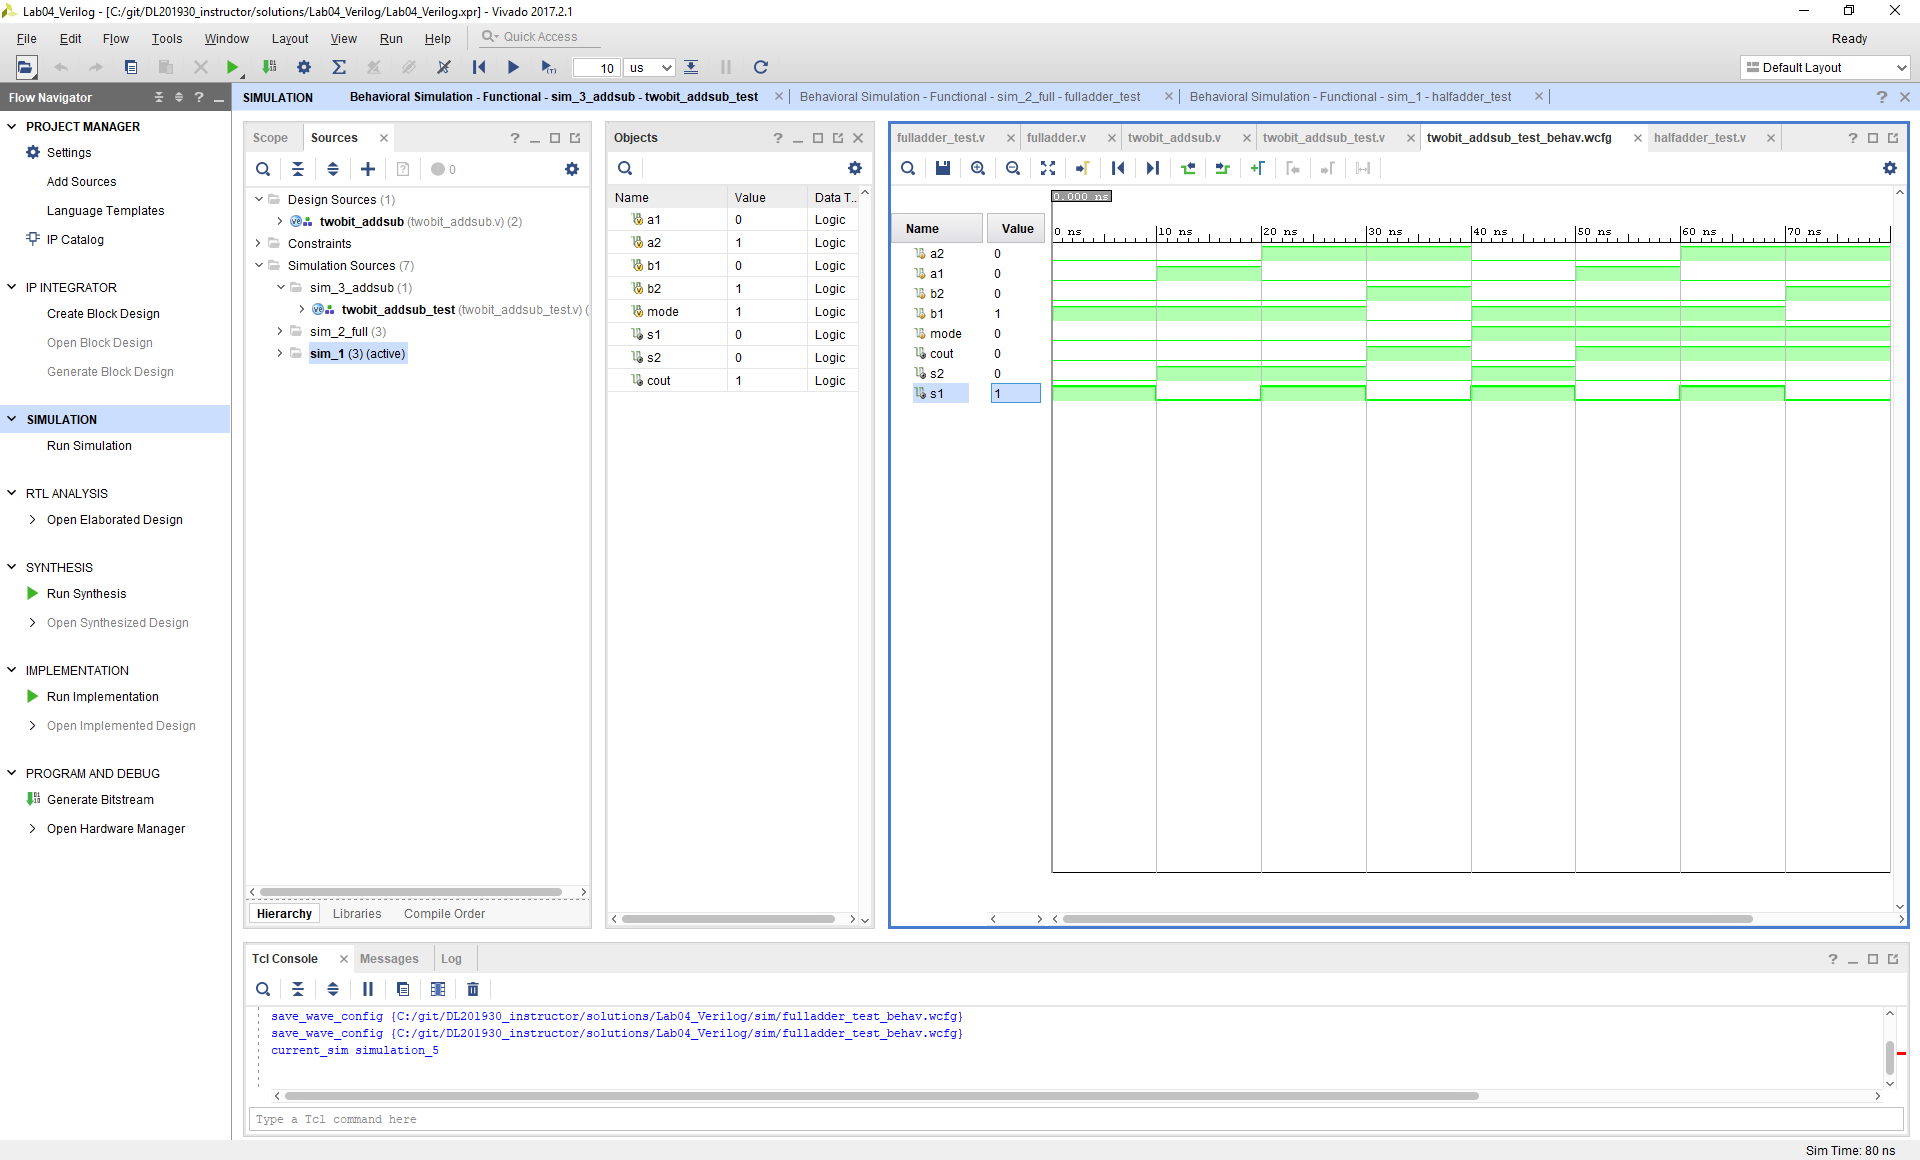
\includegraphics[width=\textwidth,trim=540 455 15 130,clip]{lab1_example_screenshot}
\caption{These are the Expected Results and the waveform of the data}
\label{fig:results_and_waveform}
\end{figure}
\end{center}

\section*{}
\section*{}
\section*{}
\section*{Screenshot}

\begin{figure}[ht]\centering
	\includegraphics[width=\textwidth,trim=175 200 175 150,clip]{Screenshot_GitHub}
	\caption{This is the screenshot from the GitHub website. This is the online history of the actions taken on my repository. My GitHub Desktop App was not letting me see my history.}
	\label{fig:Screenshot_GitHub}
\end{figure}

\begin{figure}[ht]\centering
	\includegraphics[width=\textwidth,trim=220 200 220 59,clip]{GitHub_error_ss}
	\caption{This is the screenshot from the Github Desktop App.}
	\label{fig:GitHub_error_ss}
\end{figure}

\section*{}
\section*{}
\section*{}
\section*{}
\section*{}
\section*{}

\section*{Code}

\Verilog[caption=File-included Verilog code example,label=code:file_ex]{lab1_example_code.sv}



\end{document}
